\documentclass[aspectratio=169,11pt,t]{beamer}
% ============================================================
%  ksa-cs-v2: ksa-cs-lecture-template.tex 스타일 + 한글, v2 덱(16:9)용.
%    - 짙은 네이비 헤드라인 (섹션 이름 + 프레임마다 점)
%    - 꽉 찬 파란 제목 막대, 둥근 그림자 블록
%    - 한글: Noto Sans CJK KR (fontspec)
%  사용:
%    \documentclass[aspectratio=169,11pt,t]{beamer}
%    \input{<..>/theme/ksa-cs-v2.tex}
%  ksa-theme.tex 의 매크로(\kb \kq, ksablue/ksared 등)도 같은 이름으로 둔다
%  -> v2 덱 본문을 거의 그대로 옮길 수 있다.
% ============================================================

\usepackage{fontspec}
\usepackage{amsmath,amssymb}
\usepackage{tikz}
\usepackage{listings}
\usepackage{graphicx}
\usepackage{booktabs}
\usepackage{varwidth}
% enumitem 은 넣지 않는다 (beamer 글머리표가 사라진다)

\defaultfontfeatures{Ligatures=TeX}
\setmainfont{Noto Sans CJK KR}
\setsansfont{Noto Sans CJK KR}
\setmonofont{Noto Sans Mono CJK KR}[Scale=0.92]
\usefonttheme{professionalfonts}

% ---------- 기본 틀 ----------
\usetheme{default}
\useinnertheme[shadow=true]{rounded}
\setbeamertemplate{navigation symbols}{}
\setbeamersize{text margin left=1em,text margin right=1em}

% ---------- 색 (템플릿 원본 값) ----------
\definecolor{navydark}{HTML}{191959}
\definecolor{navydim}{HTML}{8888B0}
\definecolor{navytitle}{HTML}{262686}
\definecolor{navyblue}{HTML}{3333B2}
\definecolor{blockbodybg}{HTML}{E9E9F3}
\definecolor{examplegreen}{HTML}{006000}
\definecolor{examplebg}{HTML}{E5EFE5}
\definecolor{alertred}{HTML}{BF0000}
\definecolor{alertbg}{HTML}{F9E5E5}
% ksa-theme.tex 와 같은 이름 (본문 호환)
\colorlet{ksablue}{navytitle}
\colorlet{ksabluedk}{navydark}
\definecolor{ksagold}{HTML}{D6CBB1}
\definecolor{ksagolddk}{HTML}{A9976B}
\colorlet{ksared}{alertred}
\definecolor{ksagray}{HTML}{5B5B5B}

\setbeamercolor{structure}{fg=navyblue}
\setbeamercolor{alerted text}{fg=alertred}
\setbeamercolor{frametitle}{bg=navytitle,fg=white}
\setbeamercolor{title}{fg=white,bg=navytitle}
\setbeamercolor{block title}{bg=navytitle,fg=white}
\setbeamercolor{block body}{bg=blockbodybg,fg=black}
\setbeamercolor{block title example}{bg=examplegreen,fg=white}
\setbeamercolor{block body example}{bg=examplebg,fg=black}
\setbeamercolor{block title alerted}{bg=alertred,fg=white}
\setbeamercolor{block body alerted}{bg=alertbg,fg=black}
\setbeamercolor{item}{fg=navyblue}
\setbeamertemplate{itemize item}[circle]
\setbeamertemplate{itemize subitem}[triangle]

% ---------- 헤드라인: miniframes (섹션 이름 + 점) ----------
\useoutertheme[subsection=false]{miniframes}
\setbeamerfont{section in head/foot}{size=\tiny}
\setbeamercolor{section in head/foot}{bg=navydark,fg=white}
\setbeamercolor{mini frame}{fg=white}
\setbeamertemplate{mini frames}[circle]

% ---------- 제목 막대: 폭 꽉 채움, 두 줄까지 ----------
\setbeamerfont{frametitle}{size=\normalsize,series=\bfseries}
\setbeamertemplate{frametitle}{%
  \nointerlineskip
  \begin{beamercolorbox}[wd=\paperwidth,ht=2.7ex,dp=1.1ex,leftskip=.3cm,rightskip=.3cm]{frametitle}%
    \usebeamerfont{frametitle}\insertframetitle
  \end{beamercolorbox}}

% ---------- 쪽 번호: 오른쪽 아래 ----------
\setbeamertemplate{footline}{%
  \hfill
  {\color{navydim}\scriptsize\insertframenumber\,/\,\inserttotalframenumber}%
  \hspace{3mm}\vspace{2mm}%
}

% ---------- 표지: 템플릿처럼 헤드라인은 그대로, 가운데 둥근 그림자 상자에 제목 한 줄 ----------
% 덱에서:  {\setbeamertemplate{footline}{}\begin{frame}[c,noframenumbering]\titlepage\end{frame}}
\setbeamercolor{title}{fg=white,bg=navyblue}
\makeatletter
\setbeamertemplate{title page}{%
  \vfill
  \centering
  \begin{minipage}{0.84\paperwidth}
  \begin{beamercolorbox}[wd=\linewidth,sep=7pt,center,rounded=true,shadow=true]{title}
    {\usebeamerfont{title}\inserttitle\par}%
    \ifx\insertsubtitle\@empty\else\vskip0.4em{\usebeamerfont{subtitle}\insertsubtitle\par}\fi
  \end{beamercolorbox}
  \end{minipage}\par\vskip1.6em
  {\usebeamerfont{author}\color{navytitle}\insertauthor\par}\vskip0.3em
  {\usebeamerfont{institute}\color{ksagray}\insertinstitute\par}
  \vfill
}
\makeatother
\setbeamerfont{title}{series=\bfseries,size=\Large}
\setbeamerfont{subtitle}{size=\normalsize}
\setbeamerfont{author}{size=\normalsize}
\setbeamerfont{institute}{size=\small}

% ksa-theme 호환: 덱이 \renewcommand{\ksacredit}{..} 를 해도 되게 (꼬리말에는 안 쓴다)
\newcommand{\ksacredit}{}

% ---------- 강조 ----------
\newcommand{\hl}[1]{\textcolor{alertred}{#1}}
\newcommand{\hlb}[1]{\textcolor{navyblue}{#1}}
\newcommand{\kb}[1]{\textbf{\color{ksablue}#1}}
\newcommand{\kq}[1]{\textbf{\color{ksared}#1}}

% ---------- 파이썬 코드 (템플릿과 같은 색) ----------
\definecolor{codekw}{HTML}{0033B3}
\definecolor{codebuiltin}{HTML}{BF0000}
\definecolor{codestr}{HTML}{067D17}
\definecolor{codecomment}{HTML}{8C8C8C}
\definecolor{codenum}{HTML}{1750EB}
\lstdefinestyle{py}{
  language=Python, basicstyle=\ttfamily\scriptsize,
  keywordstyle=\color{codekw}\bfseries, stringstyle=\color{codestr},
  commentstyle=\color{codecomment}\itshape, numberstyle=\color{codenum},
  emph={print,len,range,sum,input,int,str,float,list,dict,append,remove,sorted,abs,min,max},
  emphstyle=\color{codebuiltin}, showstringspaces=false, keepspaces=true,
  columns=fixed, basewidth=0.52em, aboveskip=1mm, belowskip=1mm, xleftmargin=2mm,
  breaklines=true
}
\lstset{style=py}

% 원본 자료: slides/v2/ml1/week11/gru/ (data.py · make_figs.py · exp_char.py · lab/) -- 그림은 거기 figs/ 를 그대로 쓴다
\setbeamerfont{author}{size=\normalsize}
\setbeamerfont{institute}{size=\small}
\graphicspath{{../../../v2/ml1/week11/gru/figs/}{../../../v2/ml1/week11/lstm/figs/}{../../../assets/}}
\definecolor{ksagreen}{HTML}{2A9D8F}
\makeatletter
\newcommand{\markpage}[1]{\protected@write\@auxout{}{\string\newlabel{#1}{{\the\c@framenumber}{}}}\hypertarget{#1}{}}
\newcommand{\pref}[1]{\hyperlink{#1}{\textcolor{ksagolddk}{(p.\ref{#1})}}}
\makeatother

\renewcommand{\ksacredit}{Machine Learning and Deep Learning \,\textperiodcentered\, GRU}
\title{GRU 게이트 순환 유닛 (Gated Recurrent Unit)}
\subtitle{문 두 개, 기억 하나로 줄인 LSTM}
\author{Machine Learning and Deep Learning}
\institute{한국과학영재학교 (KSA)}
\date{}
\begin{document}
{\setbeamertemplate{footline}{}\begin{frame}[c,noframenumbering]\titlepage\end{frame}}

\section{질문}
% --- 오늘의 질문
\begin{frame}{오늘의 질문: 문 세 개, 기억 두 개, 다 필요할까?}
\vfill
\centering
\renewcommand{\arraystretch}{1.5}
{\large\begin{tabular}{lll}
 & LSTM (1997, 2000) & ?\\\hline
문 & 잊기 $f$ · 적기 $i$ · 꺼내기 $o$ \quad \textbf{3개} & \kb{2개}\\
기억 & 셀 상태 $c$ + 출력 $h$ \quad \textbf{2개} & \kb{$h$ 하나}\\
가중치 묶음 & 4묶음 (RNN 의 4배) & \kb{3묶음}
\end{tabular}}\vskip0.8em
{\large 잊는 만큼 적으면 되지 않을까? \quad $f$ 와 $i$ 를 \textbf{하나로} 묶자}\\[0.3em]
{\small Cho 외 (2014): 다음 시간 Seq2Seq 의 바로 그 번역 논문에서 함께 나왔다}
\vfill
\note{지난 시간 LSTM은 문이 세 개, 잊는 문, 적는 문, 꺼내는 문이 있었고, 기억도 셀 상태 c와 출력 h 두 개였습니다. 가중치는 기본 RNN의 4배였죠. 이게 다 꼭 필요할까요? 2014년 조경현 교수 팀은 이렇게 생각했습니다. 기억을 지우는 만큼 새로 적으면 되지 않을까? 그러면 잊는 문과 적는 문을 하나로 묶을 수 있습니다. 그렇게 문 두 개, 기억 하나로 줄인 것이 오늘 배울 GRU입니다. 이 구조는 다음 시간에 배울 Seq2Seq 번역 논문에서 함께 나왔습니다.}
\end{frame}

\section{GRU}
% --- 그림
\begin{frame}{GRU: 지키는 만큼 덜 적는다}
\markpage{cell}
\vfill
\centering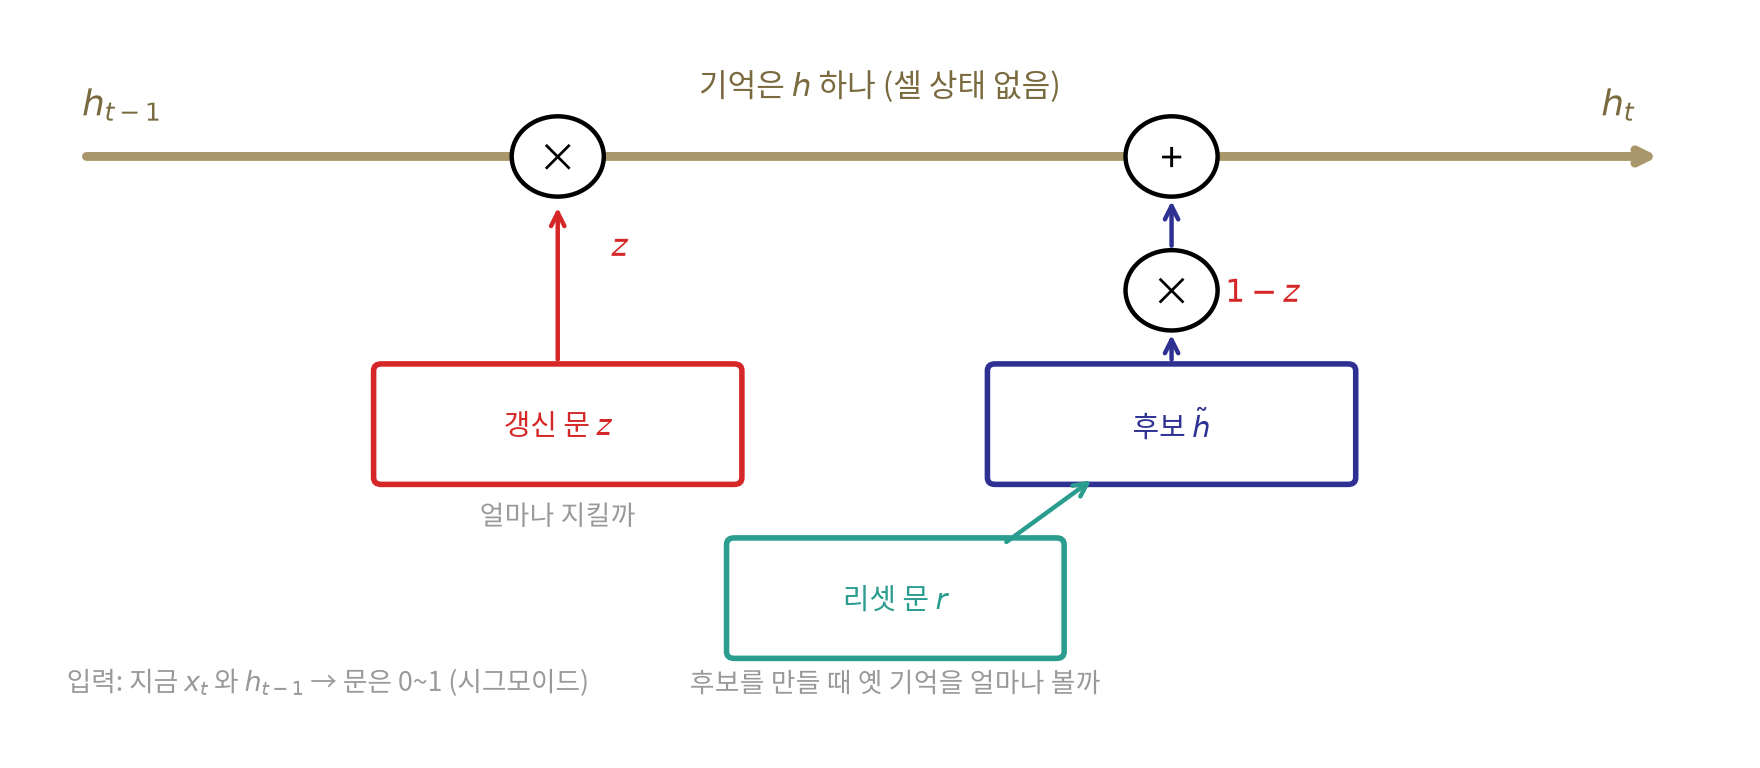
\includegraphics[width=0.8\linewidth]{gru_cell.png}\par\vskip0.2em
{\large \textcolor{ksared}{갱신 문 $z$}: 옛 기억을 $z$ 만큼 지키고, 나머지 $1 - z$ 만큼 새 후보로 채운다}\\[0.2em]
{\large \textcolor{ksagreen}{리셋 문 $r$}: 후보를 만들 때 옛 기억을 얼마나 참고할지}
\vfill
\note{GRU 그림입니다. 위쪽 노란 선이 기억 h입니다. LSTM과 달리 셀 상태가 따로 없고 h 하나가 기억이자 출력입니다. 빨간 갱신 문 z는 옛 기억을 얼마나 지킬지 정합니다. z만큼 지키고, 남은 1 빼기 z만큼은 새 후보로 채웁니다. 지키는 만큼 덜 적는 거죠. 초록 리셋 문 r은 새 후보를 만들 때 옛 기억을 얼마나 참고할지 정합니다. r이 0이면 옛 기억을 무시하고 지금 입력만 보고 후보를 만듭니다.}
\end{frame}

% --- 식
\begin{frame}{식으로}
\markpage{formula}
\vfill
\centering
{\large\[ \textcolor{ksared}{\mathbf{z}_t} = \sigma(W_z[\mathbf{h}_{t-1}, \mathbf{x}_t]) \qquad \textcolor{ksagreen}{\mathbf{r}_t} = \sigma(W_r[\mathbf{h}_{t-1}, \mathbf{x}_t]) \]
\[ \tilde{\mathbf{h}}_t = \tanh(W_h[\textcolor{ksagreen}{\mathbf{r}_t} \odot \mathbf{h}_{t-1}, \mathbf{x}_t]) \]}\vskip0.2em
{\LARGE\[ \mathbf{h}_t = \textcolor{ksared}{\mathbf{z}_t} \odot \mathbf{h}_{t-1} + (1 - \textcolor{ksared}{\mathbf{z}_t}) \odot \tilde{\mathbf{h}}_t \]}\vskip0.2em
\renewcommand{\arraystretch}{1.2}
{\normalsize\begin{tabular}{ll}
$\sigma$: 0 $\sim$ 1 & 칸마다 따로 정한다 \quad $\odot$ = 칸별 곱 \quad 편향은 생략\\
방향 주의 & 원 논문 · PyTorch 와 같은 방향 ($z$ = 지키는 비율). 반대로 쓰는 책도 있다
\end{tabular}}
\vfill
\note{식으로 쓰면 이렇습니다. 갱신 문 z와 리셋 문 r은 LSTM의 문처럼 이전 기억 h와 지금 입력 x를 이어 붙여 가중치를 곱하고 시그모이드를 씌웁니다. 후보 h 틸드는 이전 기억에 리셋 문을 칸별로 곱한 뒤 입력과 이어 붙여 tanh를 씌웁니다. 새 기억은 이전 기억에 z를 곱한 것과 후보에 1 빼기 z를 곱한 것의 합입니다. 두 비율의 합이 항상 1이니, 지키는 만큼 덜 적습니다. 주의할 점 하나. 여기서는 원 논문과 PyTorch처럼 z를 지키는 비율로 썼습니다. z와 1 빼기 z를 반대로 쓰는 책과 블로그도 많으니, 읽을 때 어느 쪽인지 확인하세요.}
\end{frame}

% --- 손 계산 1
\begin{frame}{손으로 한 번: 갱신 문}
\markpage{hand}
\vfill
\centering
{\large 이전 기억 $h_{t-1} = 0.8$ \qquad 후보 $\tilde{h} = -0.2$ \qquad 갱신 문 $z = 0.9$}\vskip0.4em
{\LARGE\[ h_t = \underbrace{0.9 \times 0.8}_{\text{keep 90\%}} + \underbrace{0.1 \times (-0.2)}_{\text{write 10\%}} = 0.72 - 0.02 = \kb{0.70} \]}\vskip0.2em
\renewcommand{\arraystretch}{1.4}
{\large\begin{tabular}{lll}
 & 지키기 & 적기\\\hline
LSTM (지난 시간 예) & $f = 0.9$ & $i = 0.5$ \quad (따로 정한다)\\
GRU & $z = 0.9$ & $1 - z = \kb{0.1}$ \quad (자동으로 정해진다)
\end{tabular}}\\[0.5em]
{\large 90\% 를 지키면 새 내용은 10\% 만 들어간다 \quad $h$ 는 늘 옛 기억과 후보의 \textbf{가중 평균}}
\vfill
\note{기억이 한 칸인 경우로 계산해 봅니다. 이전 기억이 0.8, 후보가 마이너스 0.2, 갱신 문이 0.9입니다. 새 기억은 0.9 곱하기 0.8, 0.72에 0.1 곱하기 마이너스 0.2, 마이너스 0.02를 더해 0.70입니다. 지난 시간 LSTM 손 계산과 비교해 봅시다. LSTM은 잊는 문 0.9로 지키면서 적는 문 0.5로 새 내용을 절반 더할 수 있었고, 그래서 기억이 점점 커질 수도 있었습니다. GRU는 90퍼센트를 지키면 새 내용은 자동으로 10퍼센트만 들어갑니다. 지키기와 적기를 따로 정할 수 없는 대신, 가중치 한 묶음을 아꼈습니다. 그리고 h가 늘 옛 기억과 후보의 가중 평균이라, 0에서 출발하면 언제나 마이너스 1과 1 사이, tanh 범위 안에 머뭅니다.}
\end{frame}

% --- 손 계산 2
\begin{frame}{손으로 한 번: 리셋 문}
\vfill
\centering
{\large 후보 \quad $\tilde{h} = \tanh(\,w\,x + u\,(\textcolor{ksagreen}{r} \, h_{t-1})\,)$ \qquad $x = 1, \ w = 0.5, \ u = 2, \ h_{t-1} = 0.8$}\vskip0.6em
\renewcommand{\arraystretch}{1.6}
{\Large\begin{tabular}{lll}
\textcolor{ksagreen}{$r = 1$} & $\tanh(0.5 + 1.6) = \tanh 2.1$ & $= 0.97$ \quad 옛 기억이 섞인 후보\\
\textcolor{ksagreen}{$r = 0$} & $\tanh(0.5 + 0) = \tanh 0.5$ & $= \kb{0.46}$ \quad 지금 입력만 본 후보
\end{tabular}}\vskip0.8em
{\large $r \approx 0$: ``지난 내용은 잊고 새로 시작'' \quad 예: 새 문장, 새 단어의 첫 글자}\\[0.3em]
{\small 리셋 문은 후보만 바꾼다. 옛 기억을 실제로 얼마나 버릴지는 여전히 $z$ 가 정한다}
\vfill
\note{리셋 문도 숫자로 봅시다. 후보는 지금 입력에 w를 곱한 것과 옛 기억에 r과 u를 곱한 것을 더해 tanh를 씌웁니다. 입력 1, w 0.5, u 2, 옛 기억 0.8이라고 합시다. r이 1이면 0.5 더하기 1.6, tanh 2.1, 0.97로 옛 기억이 크게 섞인 후보가 나옵니다. r이 0이면 옛 기억이 지워져 tanh 0.5, 0.46, 지금 입력만 본 후보가 됩니다. r을 0 쪽으로 두면 지난 내용은 잊고 새로 시작하는 후보를 만드는 겁니다. 새 문장이나 새 단어가 시작될 때 쓸모 있겠죠. 다만 리셋 문은 후보만 바꿉니다. 옛 기억을 실제로 얼마나 버리고 후보로 바꿀지는 여전히 갱신 문 z가 정합니다.}
\end{frame}

% --- 대응
\begin{frame}{LSTM 과 나란히}
\vfill
\centering
\renewcommand{\arraystretch}{1.6}
{\large\begin{tabular}{lll}
 & LSTM & GRU\\\hline
지키기 & 잊는 문 $f$ & 갱신 문 $z$\\
적기 & 적는 문 $i$ (따로) & $1 - z$ \quad \kb{($f$ 와 $i$ 를 묶음)}\\
꺼내기 & 꺼내는 문 $o$ & 없음: 기억을 \textbf{그대로} 보여 준다\\
후보 만들 때 & 이전 출력 $h$ 를 다 본다 & 리셋 문 $r$ 만큼만 본다\\
기억 & $c$ (안) + $h$ (밖) & $h$ 하나\\
상태 넘기기 & \texttt{(h, c)} & \texttt{h}
\end{tabular}}
\vfill
\note{LSTM과 나란히 놓아 봅시다. 지키기는 LSTM의 잊는 문, GRU의 갱신 문이 맡습니다. 적기는 LSTM에서는 적는 문이 따로 정하지만, GRU는 1 빼기 z로 자동으로 정해집니다. 잊는 문과 적는 문을 하나로 묶은 겁니다. 꺼내는 문은 GRU에 없습니다. 기억을 감추지 않고 그대로 보여 줍니다. 대신 후보를 만들 때 옛 기억을 얼마나 볼지 정하는 리셋 문이 있습니다. 기억도 LSTM은 안쪽 셀 상태와 바깥 출력 두 개였지만 GRU는 h 하나라서, PyTorch에서 다음 칸에 넘기는 상태도 h 하나입니다.}
\end{frame}

\section{기억}
% --- 왜 오래
\begin{frame}{왜 오래 기억할 수 있나}
\vfill
\centering
{\LARGE\[ \mathbf{h}_t = \textcolor{ksared}{\mathbf{z}_t} \odot \mathbf{h}_{t-1} + \cdots \qquad \Rightarrow \qquad \text{지름길로 } \mathbf{z}_t \text{ 만 곱해진다} \]}\vskip0.4em
{\large LSTM 의 $c_t = f \odot c_{t-1} + \cdots$ 와 같은 \kb{더하기} 경로 \quad 행렬도 tanh 도 없다}\\[0.6em]
{\large 기억해야 할 때 $z \approx 1$ 로 학습하면 \quad $0.999^{100} \approx \kb{90\%}$ \quad 기울기도 그대로 전달}\\[0.4em]
{\small 기본 RNN: 걸음마다 $W_h$ 와 $\tanh'$ 을 곱한다 $\to$ $0.9^{100} \approx 0.003\%$}
\vfill
\note{GRU도 LSTM처럼 오래 기억할 수 있습니다. 새 기억에는 이전 기억에 z를 곱한 항이 그대로 더해집니다. 이 지름길로는 행렬도 tanh도 없이 z만 곱해집니다. LSTM의 셀 상태가 잊는 문만 곱해지며 이어지는 것과 같은 더하기 경로입니다. 그래서 기억해야 할 때 z를 1에 가깝게 학습하면, 0.999의 100제곱처럼 기억과 기울기가 거의 그대로 100걸음을 갑니다. 기본 RNN이 걸음마다 W_h와 tanh의 기울기를 곱해 0.9의 100제곱, 0.003퍼센트로 사라졌던 것과 대비됩니다.}
\end{frame}

% --- 가중치 세기
\begin{frame}{손으로 세기: 가중치는 LSTM 의 $\frac34$}
\markpage{count}
\vfill
\begin{columns}[c]
\column{0.5\linewidth}\centering
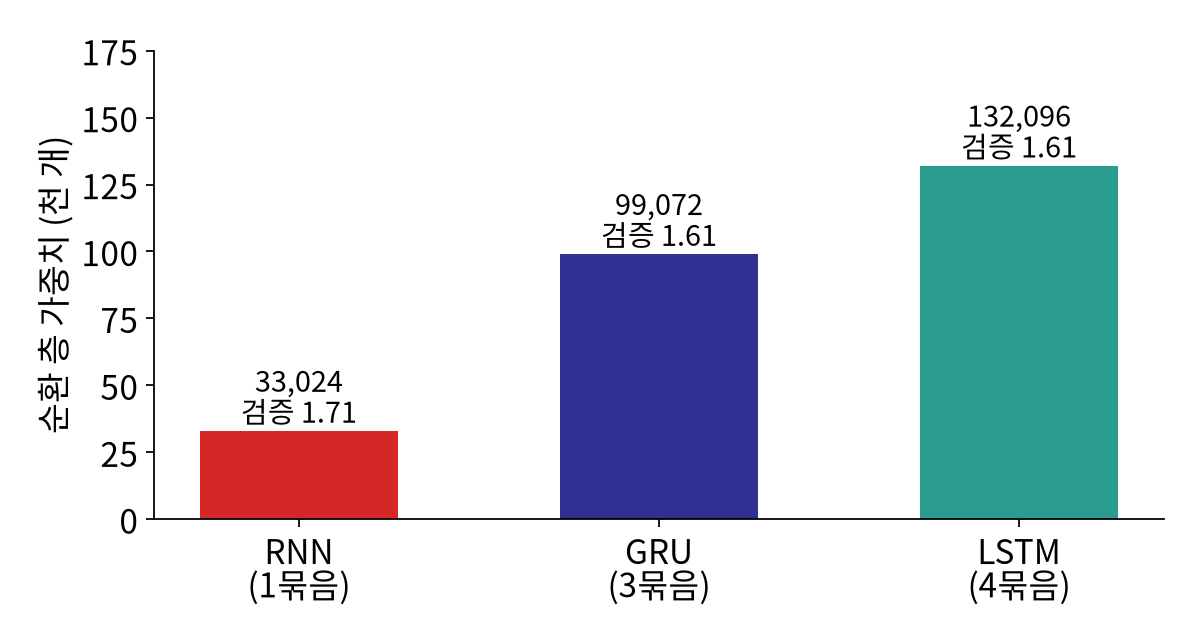
\includegraphics[width=\linewidth]{gru_params.png}
\column{0.48\linewidth}
{\large 묶음 하나 (입력 $x$ 칸, 은닉 $h$ 칸):}\\[0.2em]
{\large $h \times (x + h)$ + 편향}\\[0.6em]
\renewcommand{\arraystretch}{1.4}
{\large\begin{tabular}{ll}
RNN & 1묶음\\
GRU & \kb{3묶음}: $z$, $r$, 후보\\
LSTM & 4묶음: $f$, $i$, $o$, 후보
\end{tabular}}\\[0.6em]
{\small 입력 128 · 은닉 128, PyTorch (편향 2개): \quad $3 \times 33{,}024 = 99{,}072$}
\end{columns}
\vfill
\note{가중치를 세 봅시다. 묶음 하나는 은닉 칸 수 곱하기 입력 칸과 은닉 칸의 합에 편향을 더한 것입니다. 기본 RNN은 1묶음, GRU는 갱신 문, 리셋 문, 후보로 3묶음, LSTM은 세 문과 후보로 4묶음입니다. 그래서 GRU의 가중치는 LSTM의 4분의 3입니다. 입력과 은닉이 128칸이면 PyTorch는 편향을 두 개 두어서 묶음 하나가 33,024개, GRU는 그 3배인 99,072개, LSTM은 132,096개입니다. 막대 위의 검증 손실은 다음 쪽 실험 결과입니다.}
\end{frame}

\section{실험}
% --- 실험
\begin{frame}{실험: 셰익스피어 글자 모델, RNN vs LSTM vs GRU}
\markpage{exp}
\vfill
\centering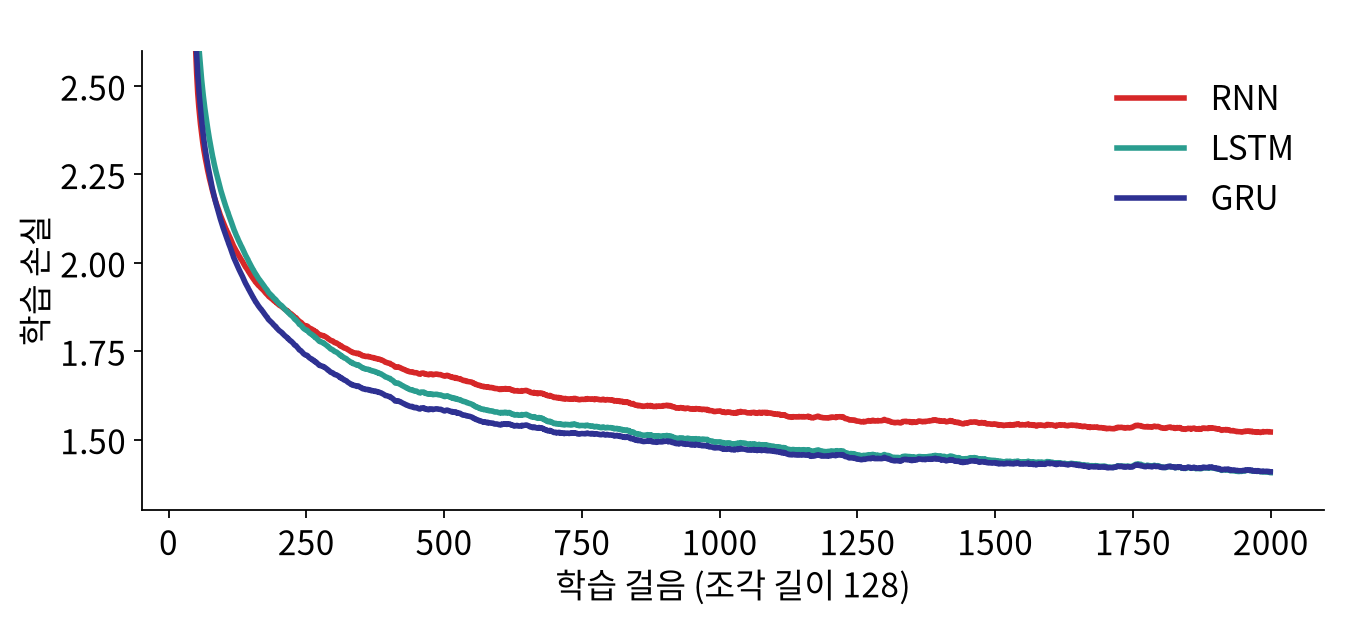
\includegraphics[width=0.56\linewidth]{gru_curve.png}\par\vskip0.2em
\renewcommand{\arraystretch}{1.2}
{\large\begin{tabular}{lccc}
검증 손실 (뒤 10\% 글) & 조각 64 & 조각 128 & 가중치\\\hline
RNN & 1.74 & 1.71 & 3.3만\\
LSTM & \kb{1.64} & \kb{1.61} & 13.2만\\
GRU & 1.66 & \kb{1.61} & 9.9만
\end{tabular}}
\vfill
\note{지난 시간 셰익스피어 글자 모델에 GRU를 더했습니다. 은닉 크기 128, 2000걸음, 같은 조건입니다. 학습 곡선에서 GRU는 처음에 LSTM보다도 조금 빨리 내려갑니다. 학습에 쓰지 않은 뒤 10퍼센트 글로 잰 검증 손실은 조각 길이 64에서 LSTM 1.64, GRU 1.66, 128에서는 둘 다 1.61입니다. RNN의 1.71보다 확실히 낫고, 가중치는 LSTM의 4분의 3으로 거의 같은 성능을 냈습니다.}
\end{frame}

% --- 무엇을 쓸까
\begin{frame}{LSTM 과 GRU, 무엇을 쓸까?}
\vfill
\centering
\renewcommand{\arraystretch}{1.5}
{\large\begin{tabular}{ll}
Chung 외 (2014) & 음악 · 음성: GRU $\approx$ LSTM, 둘 다 기본 RNN 보다 낫다\\
Jozefowicz 외 (2015) & 구조 1만 개 넘게 비교: GRU 가 앞선 과제가 많았지만,\\
 & 잊는 문 편향을 1 로 둔 LSTM 이 거의 따라잡았다\\
우리 실험 & 검증 손실 같음 (1.61), 가중치는 GRU 가 $\frac34$
\end{tabular}}\vskip0.8em
{\large 정답은 없다: 데이터가 적거나 빨라야 하면 GRU, 아니면 둘 다 해 보기}\\[0.3em]
{\small PyTorch: \texttt{nn.LSTM} $\leftrightarrow$ \texttt{nn.GRU} 한 줄 바꾸기 (상태만 \texttt{(h, c)} $\to$ \texttt{h})}
\vfill
\note{그럼 무엇을 쓸까요? 2014년 정준영, 조경현 등의 비교에서는 음악과 음성 데이터에서 GRU와 LSTM이 비슷했고, 둘 다 기본 RNN보다 훨씬 나았습니다. 2015년 구글의 요제포비치, 자렘바, 수츠케버는 순환 구조 1만 개 넘게를 비교했는데, GRU가 LSTM보다 나은 과제가 많았지만 LSTM의 잊는 문 편향을 1로 두면 차이를 거의 따라잡았습니다. 우리 실험에서도 검증 손실은 같았습니다. 정답은 없습니다. 데이터가 적거나 가볍고 빨라야 하면 GRU를 먼저, 아니면 둘 다 해 보면 됩니다. PyTorch에서는 한 줄만 바꾸면 되고, 상태가 h와 c 두 개에서 h 하나로 바뀌는 것만 챙기면 됩니다.}
\end{frame}

\section{연습}
% --- 문제풀이
\begin{frame}{문제풀이}
\vfill
\begin{enumerate}
\item $h_{t-1} = 0.6$, $\tilde{h} = -0.2$, $z = 0.75$ 이면 $h_t$ 는? $z = 0$ 이면?\vskip0.8em
\item 갱신 문이 계속 0.99 면 100걸음 뒤 옛 기억은 몇 \% 남나? ($0.99^{100} \approx 0.366$)\vskip0.8em
\item 입력 100칸, 은닉 128칸인 GRU 층의 가중치 수는? (3묶음, 편향 하나로 세기) \quad 같은 크기 LSTM 과 차이는?\vskip0.8em
\item GRU 에는 꺼내는 문이 없다. 그래도 ``기억은 하되 지금 출력에는 드러내지 않기''를 하려면?
\end{enumerate}
\vfill
\note{1번 답. 0.75 곱하기 0.6, 0.45에 0.25 곱하기 마이너스 0.2, 마이너스 0.05를 더해 0.40입니다. z가 0이면 옛 기억을 다 버리고 후보 마이너스 0.2가 됩니다. 2번 답. 약 36.6퍼센트입니다. 3번 답. 묶음 하나가 128 곱하기 228에 편향 128, 29,312개이고, 3묶음이면 87,936개입니다. LSTM은 117,248개라 29,312개, 한 묶음만큼 적습니다. 4번 답. 정답이 하나는 아닙니다. 기억 h의 일부 칸에 정보를 담아 두고, 다음 층이 그 칸을 작은 가중치로 읽게 배울 수 있습니다. LSTM은 이를 꺼내는 문으로 명시적으로 하고, GRU는 다음 층에 맡기는 셈입니다.}
\end{frame}

% --- 실습
\begin{frame}{실습}
\vfill
\centering\begin{tabular}{rl}
\large 1 & 갱신 문 · 리셋 문 손 계산 0.70 · 0.46, numpy GRU 한 칸 $\to$ \texttt{nn.GRUCell} 과 비교\\[0.5em]
\large 2 & 셰익스피어 글자 모델: \texttt{nn.LSTM} vs \texttt{nn.GRU} (손실 · 가중치 · 한 걸음 시간)\\[0.5em]
\large 3 & 학습된 GRU 의 갱신 문 들여다보기 $\to$ 글 써 보기
\end{tabular}\vskip1em
Tiny Shakespeare (Karpathy, char-rnn) \\[0.4em]\href{https://colab.research.google.com/github/SuminHan/book-ml/blob/main/slides/v2/ml1/week11/gru/lab/gru.ipynb}{\textcolor{ksagolddk}{▶ Colab에서 실습 노트북 열기}}
\vfill
\note{실습은 세 부분입니다. 첫째, 갱신 문과 리셋 문 손 계산을 코드로 재현하고, numpy로 GRU 한 칸을 만들어 PyTorch GRUCell과 같은 값이 나오는지 확인합니다. 둘째, 셰익스피어 글자 모델을 LSTM과 GRU로 학습해 손실, 가중치 수, 한 걸음 시간을 비교합니다. 셋째, 학습된 GRU의 갱신 문이 글자마다 어떻게 열리고 닫히는지 들여다보고 글을 써 봅니다.}
\end{frame}

\section{정리}
% --- 정리
\begin{frame}{정리}
\vfill
\centering\large\begin{tabular}{l}
\textbf{GRU} (Cho 외 2014): 문 두 개, 기억 $h$ 하나\\[0.5em]
$h_t = \textcolor{ksared}{z} \odot h_{t-1} + (1 - \textcolor{ksared}{z}) \odot \tilde{h}$ \quad 지키는 만큼 덜 적는다 ($f$ 와 $i$ 를 묶음)\\[0.5em]
리셋 문 $r$: 후보를 만들 때 옛 기억을 얼마나 볼지 \quad 꺼내는 문은 없다\\[0.5em]
가중치 LSTM 의 $\frac34$ \quad 셰익스피어 검증 손실 1.61 (LSTM 과 같음) \quad 다음: Seq2Seq
\end{tabular}
\vfill
\note{정리합니다. GRU는 2014년 조경현 교수 팀이 낸 구조로, 문이 두 개이고 기억은 h 하나입니다. 새 기억은 옛 기억과 후보를 z 대 1 빼기 z로 섞습니다. 지키는 만큼 덜 적는, 잊는 문과 적는 문을 묶은 구조입니다. 리셋 문은 후보를 만들 때 옛 기억을 얼마나 볼지 정하고, 꺼내는 문은 없습니다. 가중치는 LSTM의 4분의 3인데, 셰익스피어 실험에서 검증 손실은 1.61로 같았습니다. 다음 시간에는 LSTM이나 GRU 두 개로 번역하는 Seq2Seq를 배웁니다.}
\end{frame}
\end{document}
